%Version 3 December 2023
% See section 11 of the User Manual for version history
%
%%%%%%%%%%%%%%%%%%%%%%%%%%%%%%%%%%%%%%%%%%%%%%%%%%%%%%%%%%%%%%%%%%%%%%
%%                                                                 %%
%% Please do not use \input{...} to include other tex files.       %%
%% Submit your LaTeX manuscript as one .tex document.              %%
%%                                                                 %%
%% All additional figures and files should be attached             %%
%% separately and not embedded in the \TeX\ document itself.       %%
%%                                                                 %%
%%%%%%%%%%%%%%%%%%%%%%%%%%%%%%%%%%%%%%%%%%%%%%%%%%%%%%%%%%%%%%%%%%%%%

%%\documentclass[referee,sn-basic]{sn-jnl}% referee option is meant for double line spacing

%%=======================================================%%
%% to print line numbers in the margin use lineno option %%
%%=======================================================%%

%%\documentclass[lineno,sn-basic]{sn-jnl}% Basic Springer Nature Reference Style/Chemistry Reference Style

%%======================================================%%
%% to compile with pdflatex/xelatex use pdflatex option %%
%%======================================================%%

%%\documentclass[pdflatex,sn-basic]{sn-jnl}% Basic Springer Nature Reference Style/Chemistry Reference Style


%%Note: the following reference styles support Namedate and Numbered referencing. By default the style follows the most common style. To switch between the options you can add or remove “Numbered” in the optional parenthesis. 
%%The option is available for: sn-basic.bst, sn-vancouver.bst, sn-chicago.bst%  
 
%%\documentclass[pdflatex,sn-nature]{sn-jnl}% Style for submissions to Nature Portfolio journals
%%\documentclass[pdflatex,sn-basic]{sn-jnl}% Basic Springer Nature Reference Style/Chemistry Reference Style
\documentclass[pdflatex,sn-mathphys-num]{sn-jnl}% Math and Physical Sciences Numbered Reference Style 
%%\documentclass[pdflatex,sn-mathphys-ay]{sn-jnl}% Math and Physical Sciences Author Year Reference Style
%%\documentclass[pdflatex,sn-aps]{sn-jnl}% American Physical Society (APS) Reference Style
%%\documentclass[pdflatex,sn-vancouver,Numbered]{sn-jnl}% Vancouver Reference Style
%%\documentclass[pdflatex,sn-apa]{sn-jnl}% APA Reference Style 
%%\documentclass[pdflatex,sn-chicago]{sn-jnl}% Chicago-based Humanities Reference Style

%%%% Standard Packages
%%<additional latex packages if required can be included here>

\usepackage{graphicx}%
\usepackage{multirow}%
\usepackage{amsmath,amssymb,amsfonts}%
\usepackage{amsthm}%
\usepackage{mathrsfs}%
\usepackage[title]{appendix}%
\usepackage{xcolor}%
\usepackage{textcomp}%
\usepackage{manyfoot}%
\usepackage{nameref}%
\usepackage{booktabs}%
\usepackage{algorithm}%
\usepackage{algorithmicx}%
\usepackage{algpseudocode}%
\usepackage{listings}%
\usepackage[singlelinecheck=false,justification=justified]{caption}
\usepackage{subcaption}
\usepackage{gensymb}

\usepackage{titlesec}
\titleformat{\section}[block]
  {\fontsize{12}{15}\bfseries}
  {S\thesection}
  {1em}
  {}
\titleformat{\subsection}[hang]
  {\fontsize{12}{15}\bfseries}
  {S\thesubsection}
  {1em}
  {}
  
\definecolor{codegreen}{rgb}{0,0.6,0}
\definecolor{codegray}{rgb}{0.5,0.5,0.5}
\definecolor{codepurple}{rgb}{0.58,0,0.82}
\definecolor{backcolour}{rgb}{0.95,0.95,0.92}

\lstdefinestyle{mystyle}{
    backgroundcolor=\color{backcolour},   
    commentstyle=\color{codegreen},
    keywordstyle=\color{magenta},
    numberstyle=\tiny\color{codegray},
    stringstyle=\color{codepurple},
    basicstyle=\ttfamily\footnotesize,
    breakatwhitespace=false,         
    breaklines=true,                 
    captionpos=b,                    
    keepspaces=true,                 
    numbers=left,                    
    numbersep=5pt,                  
    showspaces=false,                
    showstringspaces=false,
    showtabs=false,                  
    tabsize=2
}

\lstset{style=mystyle}

\usepackage{array}
\newcolumntype{P}[1]{>{\hspace{0pt}}p{#1\linewidth}}

% \usepackage[nohyphen]{underscore}
\usepackage{longtable}
%%%%

%%%%%=============================================================================%%%%
%%%%  Remarks: This template is provided to aid authors with the preparation
%%%%  of original research articles intended for submission to journals published 
%%%%  by Springer Nature. The guidance has been prepared in partnership with 
%%%%  production teams to conform to Springer Nature technical requirements. 
%%%%  Editorial and presentation requirements differ among journal portfolios and 
%%%%  research disciplines. You may find sections in this template are irrelevant 
%%%%  to your work and are empowered to omit any such section if allowed by the 
%%%%  journal you intend to submit to. The submission guidelines and policies 
%%%%  of the journal take precedence. A detailed User Manual is available in the 
%%%%  template package for technical guidance.
%%%%%=============================================================================%%%%

%% as per the requirement new theorem styles can be included as shown below
\theoremstyle{thmstyleone}%
\newtheorem{theorem}{Theorem}%  meant for continuous numbers
%%\newtheorem{theorem}{Theorem}[section]% meant for sectionwise numbers
%% optional argument [theorem] produces theorem numbering sequence instead of independent numbers for Proposition
\newtheorem{proposition}[theorem]{Proposition}% 
%%\newtheorem{proposition}{Proposition}% to get separate numbers for theorem and proposition etc.

\theoremstyle{thmstyletwo}%
\newtheorem{example}{Example}%
\newtheorem{remark}{Remark}%

\theoremstyle{thmstylethree}%
\newtheorem{definition}{Definition}%

\renewcommand{\thefigure}{S\arabic{figure}}
\renewcommand{\thetable}{S\arabic{table}}

\raggedbottom
%%\unnumbered% uncomment this for unnumbered level heads

\begin{document}

\title[Article Title]{Supplementary information for ASKCOS: an open source software suite for synthesis planning}

\author[1]{\fnm{Zhengkai} \sur{Tu}}\email{ztu@mit.edu}
\author[2]{\fnm{Sourabh J.} \sur{Choure}}\email{sjchoure@mit.edu}
\author[2]{\fnm{Mun Hong} \sur{Fong}}\email{fong410@mit.edu}
\author[2]{\fnm{Jihye} \sur{Roh}}\email{jroh99@mit.edu}
\author[3]{\fnm{Itai} \sur{Levin}}\email{itail@mit.edu}
\author[4]{\fnm{Kevin} \sur{Yu}}\email{kyu3@mit.edu}
\author[2]{\fnm{Joonyoung F.} \sur{Joung}}\email{jjoung@mit.edu}
\author[2]{\fnm{Nathan} \sur{Morgan}}\email{knathan@mit.edu}
\author[2]{\fnm{Shih-Cheng} \sur{Li}}\email{scli@mit.edu}
\author[2]{\fnm{Xiaoqi} \sur{Sun}}\email{xiaoqis@mit.edu}
\author[2]{\fnm{Huiqian} \sur{Lin}}\email{linhq@mit.edu}
\author[2]{\fnm{Mark} \sur{Murnin}}\email{murninm@mit.edu}
\author[2]{\fnm{Jordan P.} \sur{Liles}}\email{jliles24@mit.edu}
\author[5]{\fnm{Thomas J.} \sur{Struble}}\email{Thomas.Struble@bms.com}
\author[6]{\fnm{Michael E.} \sur{Fortunato}}\email{mike.fortunato@novartis.com}
\author{\fnm{Mengjie} \sur{Liu}\textsuperscript{2,}\footnote[2]{Current affiliation: AstraZeneca. Work done while at MIT.}}\email{mjliu@mit.edu}
\author[2]{\fnm{William H.} \sur{Green}}\email{whgreen@mit.edu}
\author[2]{\fnm{Klavs F.} \sur{Jensen}}\email{kfjensen@mit.edu}
\author*[1,2]{\fnm{Connor W.} \sur{Coley}}\email{ccoley@mit.edu}

\affil[1]{\orgdiv{Department of Electrical Engineering and Computer Science}, \orgname{Massachusetts Institute of Technology}, \orgaddress{\street{77 Massachusetts Ave}, \city{Cambridge}, \state{MA}, \postcode{02139}, \country{USA}}}

\affil[2]{\orgdiv{Department of Chemical Engineering}, \orgname{Massachusetts Institute of Technology}, \orgaddress{\street{77 Massachusetts Ave}, \city{Cambridge}, \state{MA}, \postcode{02139}, \country{USA}}}

\affil[3]{\orgdiv{Department of Biological Engineering}, \orgname{Massachusetts Institute of Technology}, \orgaddress{\street{77 Massachusetts Ave}, \city{Cambridge}, \state{MA}, \postcode{02139}, \country{USA}}}

\affil[4]{\orgdiv{Center for Computational Science and Engineering}, \orgname{Massachusetts Institute of Technology}, \orgaddress{\street{77 Massachusetts Ave}, \city{Cambridge}, \state{MA}, \postcode{02139}, \country{USA}}}

\affil[5]{\orgname{Bristol Myers Squibb}, \orgaddress{\street{250 Water Street, \city{Cambridge}, \state{MA}, \postcode{02141}, \country{USA}}}}

\affil[6]{\orgname{Novartis Institutes for BioMedical Research, Inc.}, \orgaddress{\street{250 Massachusetts Avenue}, \city{Cambridge}, \state{MA}, \postcode{02139}, \country{USA}}}

\maketitle

\section{Details of solubility prediction and solvent screening}\label{results_solubility}

\begin{figure}[h!]
\centering
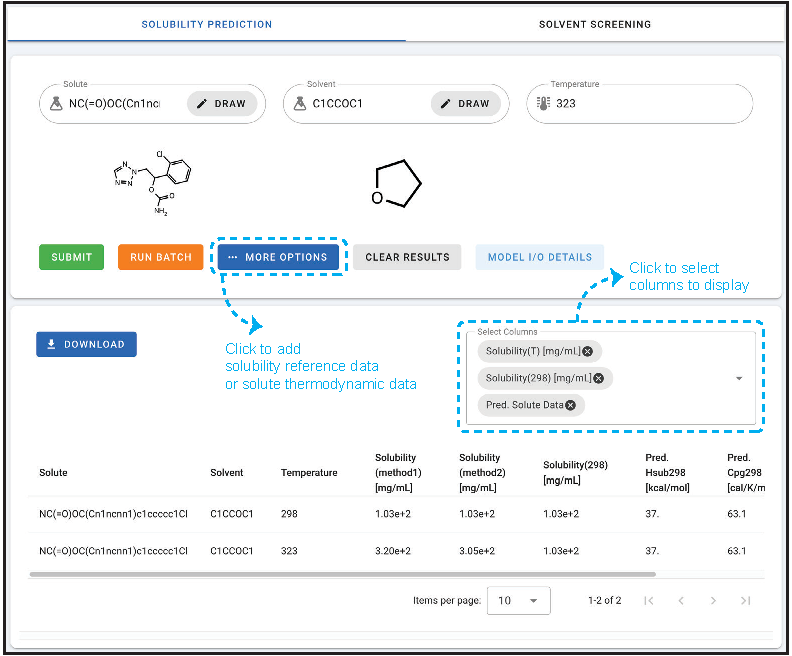
\includegraphics[width=1.0\textwidth]{media/S1.Solubility_prediction.png}
\caption{Annotated screenshot of solubility prediction results in ASKCOS. The SMILES strings of the solute and the solvent are input in the \texttt{Solute} and \texttt{Solvent} panels. The desired temperature (in K) for the solubility prediction is input in the \texttt{Temperature} panel. The predicted solubility and solvation properties of solute cenobamate, defined by the SMILES string \texttt{NC(=O)OC(Cn1ncnn1)c1ccccc1Cl}, in solvent THF, defined by the SMILES string \texttt{C1CCOC1}, at 298 K and 323 K are displayed. The property values to display (e.g., $\log S$, Abraham parameters, etc.) can be selected from the \texttt{Select Columns} panel. }\label{fig_solubility_prediction}
\end{figure}

The required input for the solubility prediction model is a solute and a solvent molecule, which are specified using a SMILES string or by using the drawing functionality (Figure \ref{fig_solubility_prediction}). After clicking the \texttt{SUBMIT} button, the predicted solubility in milligrams per milliliter is shown in a table at the bottom of the screen. The default prediction temperature is 298 K, but this can be adjusted by using the temperature field on the main screen. 
Other optional input fields are found by clicking \texttt{MORE OPTIONS}. This opens a window where users can supply a few thermodynamic parameters to improve the model's predictions. The model makes solubility predictions by first predicting the aqueous solubility at 298 K ($\log\left(S_{aq, 298\, \mathrm{K}}\right)$) and then by using other thermochemical quantities to correct that solubility to the desired solvent and temperature. The known solubility of the solute in another solvent (a reference solubility) can be given to the model to use instead of the aqueous solubility prediction, which is especially useful for solutes that have low aqueous solubility. The solubility is corrected from the reference solvent to the target solvent using ML predicted solvation free energies ($\Delta G_{solv, 298\, \mathrm{K}}$) in both solvents. $\Delta G_{solv, 298\, \mathrm{K}}$ in the target solvent can also be viewed in the output table by selecting its column in the drop down menu, which is found by clicking the arrow in the \texttt{Select Columns} field. 

The solubility in the target solvent at 298 K, $\log\left(S_{298\, \mathrm{K}}\right)$, is corrected to other temperatures using the solute's dissolution enthalpy in the target solvent, $\Delta H_{diss, \mathrm{T}}$, which in turn is estimated using ML predictions of more common thermochemical quantities in a thermodynamic cycle. These quantities include the solute's sublimation enthalpy at 298 K ($\Delta H_{sub, 298 \,\mathrm{K}}$), solid phase heat capacity at 298 K ($C_{p,s}$), gas phase heat capacity at 298 K ($C_{p,g}$), and solvation enthalpy either at 298 K ($\Delta H_{solv, 298\, \mathrm{K}}$) or the target temperature ($\Delta H_{solv,\mathrm{T}}$). All of these can be viewed in the output table by selecting them in the \texttt{Select Columns} drop down menu, similar to $\Delta G_{solv, 298\, \mathrm{K}}$. The first three quantities are predicted via correlations that use ML predicted Abraham solute parameters~\citep{chung_group_2022}. These parameters can also be viewed in the output table. Known values for the first three quantities can be given to the model to use instead of the correlations from the solute parameters. This is done using the same window as the reference solubility. 

The $\Delta H_{solv}$ used in the thermodynamic cycle can be predicted in two ways, which gives two temperature dependent solubility estimates. These are labeled ``method1" and ``method2" in the output table. The first method neglects the temperature dependence of $\Delta H_{solv}$ and uses an ML model to predict $\Delta H_{solv, 298\, \mathrm{K}}$, which is used as $\Delta H_{solv,\mathrm{T}}$. This works best for temperatures below 350 K. The second method uses an ML model to predict $\Delta G_{solv, \mathrm{T}}$, from which $\Delta H_{solv, \mathrm{T}}$ and the temperature dependent entropy ($\Delta S_{solv, \mathrm{T}}$) can be calculated. This model requires the critical temperature and density of the solvent, which limits this method's use to around 100 solvents. These temperature dependent quantities can be viewed in the output table for supported solvents. 

\begin{figure}[h!]
\centering
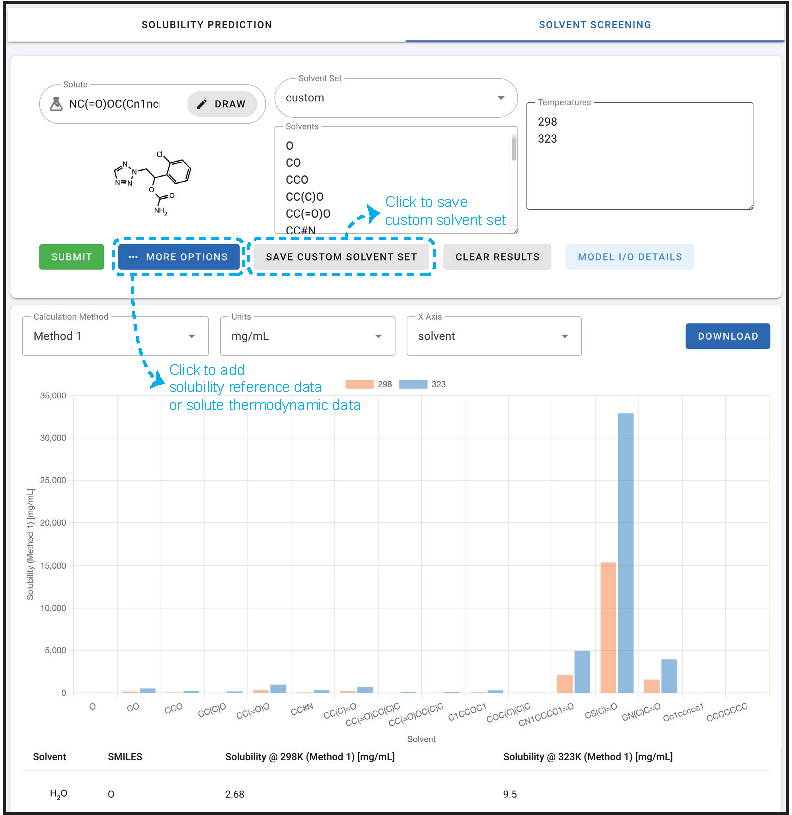
\includegraphics[width=1.0\textwidth]{media/S2.Solvent_screening.png}
\caption{Annotated screenshot of solvent screening results in ASKCOS. The SMILES string of the solute is input in the \texttt{Solute} panel. Users can select the solvents from the two predefined sets or create custom solvent sets in the \texttt{Solvent Set} panel. The desired temperatures (in K) at which to compute the solubility and solvation properties are input in the \texttt{Temperatures} panel. The predicted solubility for solute cenobamate defined by the SMILES string \texttt{NC(=O)OC(Cn1ncnn1)c1ccccc1Cl} in a custom set of solvents at 298 K and 323 K is displayed. }\label{fig_solvent_screening}
\end{figure}

A few other optional columns can be viewed in the output table, including the solubility in moles per liter, prediction uncertainty estimates, and any error or warning messages. The uncertainty estimates are the variance of predictions made by an ensemble of models. Each model in the ensemble starts with a different random initialization and is trained on the same data. An ensemble of 10, 12, and 30 models is used for $\Delta G_{solv, 298\, \mathrm{K}}$, $\Delta H_{solv, 298\, \mathrm{K}}$, and $\log\left(S_{aq, 298\, \mathrm{K}}\right)$ respectively. The prediction values in the output table for these quantities are the mean of the ensemble's predictions. 

It is also possible to use the solubility utility to make bulk predictions. Clicking the \texttt{RUN BATCH} button opens a window where a csv or json file containing input data can be uploaded. Clicking \texttt{MODEL I/O DETAILS} shows the format of this file. In the output section, there is also a \texttt{DOWNLOAD} button that allows for downloading all the results as a csv or json file. 

The solvent screening utility, as shown in Figure \ref{fig_solvent_screening}, also allows for bulk solubility predictions of a single solute in a set of solvents and temperatures. Two sets of a variety of solvents are predefined, and users can also make a custom set. The output predictions are shown in both table and chart forms. A bar chart is used if solvent is plotted on the x-axis, whereas a line chart is used if temperature is plotted on the x-axis. 

\section{Details of QM descriptor prediction}\label{results_qm}

ML has been widely used for chemical property predictions, but its performance and generalizability often depends on the availability of large datasets. However, acquiring large-scale datasets can be expensive and time-consuming in scenarios such as \emph{de novo} drug and material design. Driven by the belief that QM descriptors can provide deeper physical insights, recent studies~\citep{guan_regio-selectivity_2021,li_when_2024,stuyver2022quantum} have tried augmenting ML models with QM descriptors. It has been shown that this approach can improve the accuracy and generalizability of the model, especially when trained on smaller datasets. Thus, this method could potentially accelerate the exploration of complex reaction pathways in retrosynthesis and the prioritization of candidates in high-throughput screening.

Since calculating QM descriptors for all the molecules of interest can be very expensive, we include trained models from Li et al.'s work~\citep{li_when_2024} in ASKCOS to predict 37 general QM descriptors on the fly. These models are directed message passing neural network (D-MPNN) models trained on QM descriptors computed using $\omega$B97XD/def2-SVP//GFN2-xTB. The 37 descriptors consist of 13 atom descriptors, 4 bond descriptors, and 20 molecular descriptors. The atom descriptors include NPA charges, Parr functions, NMR shielding constants, and valence orbital occupancies. The bond descriptors consist of bond order, bond length, bonding electrons, and bond natural ionicity. The molecular descriptors encompass energy gaps, ionization potential (IP), electron affinity (EA), and dipole and quadrupole moments. For partial charge prediction, the summation is constrained by the molecule's net charge, nucleophilic/electrophilic Parr functions sum to 1, and no constraints apply to other atom or bond descriptors.

The required input for QM descriptor prediction is either a SMILES string or the use of the drawing functionality. After clicking the \texttt{SUBMIT} button, the predicted QM descriptors will be displayed in a table at the bottom of the screen. By default, only the NPA charges and Parr functions are shown. Other predicted descriptors can be displayed in the output table by selecting them from the \texttt{Select Columns} drop-down menu. Each atom and bond property of a molecule is saved in a list, with the order defined by the RDKit~\citep{RDKit} molecule object. To better visualize these descriptors, users can click the 3D visualization button in the table to view the predicted values individually (Figure \ref{fig_qm_descriptors}) for the selected molecule. In the output section, there is also a \texttt{DOWNLOAD} button that allows you to download all the results as a CSV or JSON file.

\begin{figure}[h!]
\centering
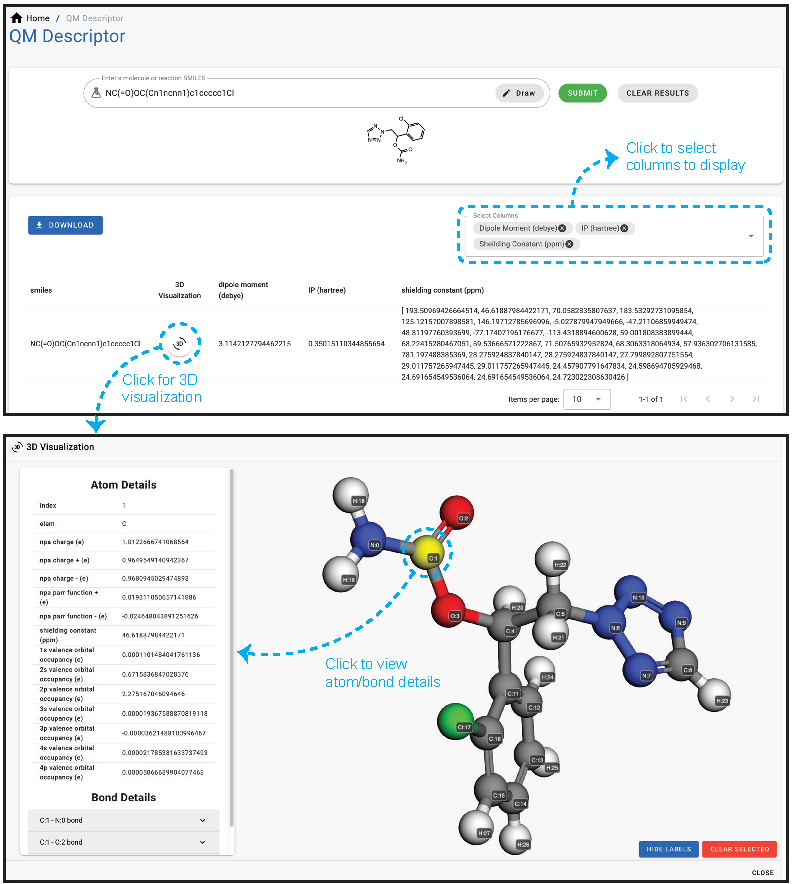
\includegraphics[width=1.0\textwidth]{media/S3.QM_feature_prediction.png}
\caption{Annotated screenshot of QM descriptor prediction results in ASKCOS. The predicted QM descriptors of cenobamate, defined by the SMILES string \texttt{NC(=O)OC(Cn1ncnn1)c1ccccc1Cl}, are displayed (top). The atom and bond descriptors can also be viewed individually with the 3D visualization page (bottom). The selected atom is highlighted in yellow, and the predicted atom properties for the selected atom is displayed on the left panel. This panel also provides predicted values for each bond connected to the selected atom.}\label{fig_qm_descriptors}
\end{figure}

\newpage
\section{Technical details of software engineering}\label{method_software}

\subsection{Refactor into a microservice-based architecture}

ASKCOS was originally developed as a pure Python 2 package beginning in 2016 to plan synthetic routes for a robotic flow chemistry platform as part of the DARPA Make-It program, with a full name of ``\textbf{A}utomated \textbf{S}ystem for \textbf{K}nowledge-based \textbf{C}ontinuous \textbf{O}rganic \textbf{S}ynthesis''. Various restful endpoints for modules were defined using the Django package, and the user interface was designed mostly using Javascript and basic Jinja templates. Since then, the number of different predictive models incorporated in ASKCOS has continued to grow. Given its long development history, the monolithic nature of ASKCOS pre-2023 presented a significant challenge in terms of maintainability and extensibility. Managing ever-changing dependencies and their deprecation (e.g., Keras, Tensorflow 1) and synchronizing environments across disparate models developed years-apart by different graduate students and postdocs became unsustainable.

The main deciding factor for a major refactor of ASKCOS was the need to resolve package dependency conflicts. As an extreme example, there is no straightforward way to run a Python program in which part of the code depends on Python 2, and another part depends on Python 3. This type of dependency conflicts became inevitable as we tried to integrate newer and more powerful modules from different contributors into ASKCOS. The de facto and somewhat obvious solution was to turn prediction modules into containerized microservices, which was exactly what has been done in the 2023 refactor, with careful decoupling and re-modularization to retain existing functionalities.

\subsection{Containerized microservices for backend modules} \label{microservices}

Prediction modules as microservices have been the cornerstone of ASKCOS, but it was not until the 2023 refactor that this philosophy was formalized. We enforce modularization and consistency of these microservices by, without loss of generality, having one containerized service per prediction module. No python function call between the modules is possible and any dependency call has to be made via http requests. For example, when the Tree Builder calls any one-step expansion model, it sends an API requests (via the API gateway) to that one-step prediction service. This preserves modularization for maintainability and extensibility in the long run, at little expense as we did not observe noticeable overhead from the conversion of function calls to API calls, especially when the services are hosted on the same machine.

The main challenges when transitioning into a microservice-based architecture was decoupling and modularization, as with code refactor in general. Once the prediction modules have been fully modularized, it is easy to replace function calls with http calls, which are now made by specialized API classes in our implementation. These modules can then be wrapped as services (i.e., as REST endpoints) using packages like FastAPI~\citep{FastAPI} and TorchServe~\citep{TorchServe}, and subsequently containerized with Docker. We refer the reader to the ASKCOS wiki~\citep{ASKCOSwiki} which has fully documented the process of converting python code into containerized services with guiding examples, under the Sections \texttt{Development-Packaging python codes as services} and \texttt{Development-Containerizing backend services}.

\subsection{Centralized API gateway}\label{method_api_gateway}

Calls to backend services are routed via the \emph{API gateway}, which is the central service in ASKCOS for API management. The API gateway is implemented with FastAPI, and consists mainly of \emph{wrappers} for routing API calls to backend services, as well as \emph{utils} which define endpoints for lightweight services such as drawing and authentication within the gateway itself. In order to take full advantage of FastAPI's capability to automatically generate API documentation based on endpoint definitions, these definitions have all been type hinted. In particular, each wrapper defines the expected input schema such as the name of the model used and other hyperparameters in a \texttt{dataclass}, which becomes visible from the auto-generated API documentation as will be illustrated in Section \nameref{method_api_usage}. The schema for the responses returned from the API gateway is defined in similar \texttt{dataclasses}. In this way, we maintain a standard pattern for all API endpoints in the gateway and make it easy to add wrappers for new prediction services: simply copy and paste the definition from an existing wrapper, and then specify the input and response schema.

We have also reworked the asynchronous workflows which are necessary for API calls from the frontend and for long-running tasks. The logic for asynchronous task management has been abstracted away and standardized as an additional endpoint, namely, \texttt{/call-async} within each wrapper. These asynchronous endpoints merely sub-call the corresponding synchronous endpoints in the same wrapper, generally with no other complication. This design keeps the effort for maintenance and extension to the minimum, while still allowing for customization if needed. The async workflows are implemented with the Celery package with RabbitMQ as the broker and Redis for storing results.

\subsection{Frontend}

% Two paragraphs, talking about the feature/techs, design choices and rational.

The ASKCOS frontend is implemented in Vue 3~\citep{Vue} which offers a more flexible, maintainable, and performant architecture. Vue 3, with its composition API and enhanced reactivity system, allows developers to create scalable components and modularize code more effectively. In the context of ASKCOS, Vue 3 serves as the foundation for a dynamic user interface, where complex chemical retrosynthesis data can be seamlessly displayed and interacted with. The integration of Vuetify~\citep{Vuetify}, a robust Material Design component library, ensures a visually cohesive and responsive user interface. Vuetify components are highly customizable, enabling developers to build feature-rich and intuitive user interfaces while adhering to modern web standards. This synergy of Vue 3 and Vuetify helps create an engaging user experience that can handle complex data visualization (in particular, on the IPP canvas) while maintaining accessibility across various devices.

A few other tools are used for testing, application state management and routing. To ensure the reliability and robustness of this complex system, Cypress~\citep{Cypress} is employed for end-to-end testing. Cypress allows for the testing of every aspect of the application from user interaction to API calls, ensuring that ASKCOS functions as intended in real-world scenarios. Pinia~\citep{Pinia} serves as the state management tool to provide a more lightweight, modular, and type-safe approach to managing application state. This helps maintain data consistency across different components, especially in handling chemical datasets and user interactions. Furthermore, Vue Router~\citep{VueRouter} integrates seamlessly with the Vue 3 framework, managing complex navigational patterns, enabling smooth transitions between different sections of the application without reloading the page. These technologies together form the backbone of the ASKCOS web platform, ensuring high performance, reliability, and ease of use for chemists and researchers accessing the platform.

\subsection{Application monitoring and logging}

% Two paragraphs, talking about the feature/techs, design choices and rationale.

Several utilities have been designed to help monitor application status while ASKCOS is running. From the \texttt{Server Status} page of the ASKCOS user interface, users can see a status summary of the services for the celery workers, the database, and prediction modules. For the celery services, the status summary shows the numbers of their pending tasks as well as of available and busy workers. For the data collections (e.g., reactions, templates, and buyable building blocks) which are stored in the Mongo database, a description of each collection and the number of documents imported during database seeding are displayed. For backend services, metadata including model names and descriptions are populated from the config file used to deploy and start ASKCOS. The service status (online vs. offline) is checked with API calls and updated upon refresh.

The logs of the API calls made from the frontend are accessible from the \texttt{Logs} page, which can be particularly helpful for debugging. The storage of such logs is made possible by Pinia which allows a state to be shared across components and pages. When a user performs an action on any ASKCOS page, if requests to the backend APIs are made, Pinia can relay information about these requests to the \texttt{Logs} page. The logs can be cleared by refreshing any page in ASKCOS.

For superusers, another useful API endpoint is \texttt{/api-logging/get}, which counts the number of API calls to each endpoint and aggregates by date. It provides succinct statistics of the most used features in ASKCOS to help superusers optimize the deployment, e.g., by increasing the number of celery workers for more frequently used modules.

\section{Advanced features}\label{advanced_features}

\subsection{User-friendly and customizable deployment}\label{method_deployment}

ASKCOS can be deployed from scratch with the following five commands:
\begin{lstlisting}[language=bash]
$ mkdir ASKCOSv2
$ cd ASKCOSv2
$ git clone git@gitlab.com:mlpds_mit/askcosv2/askcos2_core.git
$ cd askcos2_core
$ make deploy
\end{lstlisting}
We refer the reader to the ASKCOS wiki~\citep{ASKCOSwiki} for the full instructions, including hardware and software requirements. The last command, \texttt{make deploy}, is the main deployment command which does the following in sequence:

\begin{enumerate}
    \item cloning all other repositories under \texttt{ASKCOSv2/} based on the central config file in \texttt{askcos2\_core}, while downloading data and model checkpoints if needed;
    \item generating deployment scripts for building Docker images, starting services and stopping services based on the central config file;
    \item building Docker images for all services using the generated script;
    \item downloading database data and seeding into the Mongo database;
    \item starting all services using using the generated script.
\end{enumerate}

A single centralized config file specifies all the required configurations. It is easy to \emph{turn off} unneeded modules for users who are more resource-constrained or have interest in only a subset of modules. Partial deployment has been documented in the ASKCOS wiki, and we include several sample config files for typical use cases (e.g., retro-only and/or backend-only).

\subsection{Model retraining and integration}\label{method_retraining}

% Two paragraphs, talking about the feature/techs, design choices and rational.

A few models for one-step retrosynthesis and reaction outcome prediction have been designed for easy retraining and integration with new datasets. In particular, the retraining pipeline of the template relevance model has been streamlined. Only a list of reaction IDs and reaction SMILES are needed, and the user has the choice of either providing own train/validation/test splits, or letting the retraining engine handle the splitting. Thereafter, automated retraining and testing can be performed with the provided script (e.g., $\texttt{benchmark*.sh}$) after specifying the paths to the reaction files.

Integration of newly trained models into ASKCOS requires \emph{model archiving}, followed by updating the existing deployment config, and possibly seeding additional data into the database. Archiving models into a servable \texttt{.mar} file is done using \texttt{torch-model-archiver}, while the rest of the integration pipeline is mostly bookkeeping to place model files into the correct location and make the API gateway aware of the existence of the new model. The full process of retraining and integration has been documented in the ASKCOS wiki under the Section \texttt{Deployment-Model retraining and integration}.

\subsection{User customization}\label{method_customization}

ASKCOS provides options to customize many aspects of the application. The design of the deployment pipeline discussed in Section \nameref{method_deployment} allows users to easily customize their deployment. The complete application including the frontend and the backend is deployed by default, but if ASKCOS is being integrated with other systems where only API calls are being made and the user interface is not needed, backend-only deployment may be more suitable. Similarly, while some datasets are copied over and loaded into ASKCOS at first deployment, additional datasets can be added, or others removed, at a later date by simply invoking subroutines in the \texttt{deploy.sh} script in the \texttt{askcos2\_core} directory to modify the database. Additionally, as eluded to previously in Section \nameref{method_deployment}, superusers can chose to disable certain modules depending on usage and computational resources available.

Other aspects of the environment can be customized too, and most customizable environment (env) variables are found in the \texttt{.env.example} file. The user interface can be configured to use a different logo, for example, a company logo, and have a different welcome message which may include the company name. This is very important as ASKCOS is publicly accessible, and as such, there are no protections regarding intellectual property (IP). If users want to use ASKCOS on their proprietary, sensitive data, ASKCOS should be deployed behind their company firewalls. Customizing the user interface quickly informs users they are on their internal deployment and can safely and confidently enter potentially sensitive compound data. The superuser can also change the support email addresses (by modifying the \texttt{VITE\_CONTACT\_EMAIL} and \texttt{VITE\_SUPPORT\_EMAILS} env variables) from the default MIT support groups to internal support addresses to ensure sensitive data is not shared outside of the company.
 
Many companies have policies that block applications requesting data outside of their firewalls to safeguard intellectual property. ASKCOS has only one external lookup, calling on the NIH name resolving service~\citep{NIHNameResolver} to convert a compound name to its corresponding SMILES string. This service can be quickly disabled on each page by clicking the icon beside the target input area. It can permanently be disabled on deployment by setting the env variable \texttt{VITE\_ENABLE\_SMILES\_RESOLVER} to False.

ASKCOS allows users to ban chemicals and reactions. These lists are specific to that user account and not global. This allows users to ban compounds or reactions that are patented, that may be toxic or harmful, or that are otherwise considered undesirable. Chemicals or reactions can be added to the ban list directly from the IPP. Banned chemicals or reactions will not appear in the predicted pathways afterwards. Users can view, add, or delete items in their ban lists on \texttt{My Banlist} page accessible from the left hand sidebar.

The \texttt{Buyables} page and backend data structures have also been enhanced to allow superusers to add important metadata such as lead time and availability to their own building blocks. These custom metadata are easily viewable during interactive planning (via the \texttt{SEARCH BUYABLES} button in the chemical node detail panel) to assist chemists' decision making. Links to the procurement website can also be added to enable easier and quicker ordering. Superusers can add buyables individually or submit a list of buyables in a file for bulk upload.

\subsection{API usage}\label{method_api_usage}

As the frontend and the backend are fully separated in ASKCOS, it is possible to send http requests directly to the API gateway, e.g., from the command line or using some client library from any programming language. Using the APIs this way may be particularly useful for integrating some of ASKCOS' predictive modules into other workflows and for batch queries, for example, by checking whether routes with buyable building blocks can be found for a given list of (possibly many) molecules. The auto-generated API documentation mentioned in Section \nameref{method_api_gateway}, which is guaranteed to be up-to-date by design, can be accessed from the browser as an interactive web page for any locally deployed ASKCOS instance. The endpoints have been organized by groups on the documentation page, and many of these endpoints have been pre-filled with working sample queries which can be easily executed with a few clicks. The interactive nature of the documentation makes it easy for experimenting with various APIs, as well as understanding their schema and performance.

We refer the readers to the ASKCOS wiki~\citep{ASKCOSwiki} for detailed and more visual illustration of the API usage, under the Section \texttt{Advanced Usage-Using the APIs directly} where python script examples for API queries have also been provided.

\section{Illustration of applying ASKCOS to FDA-approved small molecule drugs from 2019 to 2023}\label{results_fda}

We perform a case study on FDA-approved New Chemical Entities from 2019 to 2023 (New Drug Applications only) to demonstrate how a chemist may use ASKCOS to plan routes for new targets. The compilation of raw data is retrieved from the FDA website~\citep{FDAApproval}. The raw chemical names of drug components are converted to SMILES using the NIH name resolving API~\citep{NIHNameResolver}. Unresolvable names and components found in the buyable database of ASKCOS are dropped, and the remaining list of targets are deduplicated based on the canonical SMILES. The final list contains 75 unique targets in total. The raw and processed data files, as well as the scripts for data processing and for sending tree building queries are provided with instructions under \href{https://gitlab.com/mlpds\_mit/askcosv2/askcos2\_core/-/tree/main/examples}{https://gitlab.com/mlpds\_mit/askcosv2/askcos2\_core/-/tree/main/examples}.

\subsection{Initial automated tree building with typical settings}

As a baseline, we first query the MCTS endpoint with typical search settings. Specifically, Pistachio-trained and Reaxys-trained template relevance models are used simultaneously for one-step retrosynthetic expansion, both with a maximum of 1,000 templates and a maximum cumulative template probability of 0.999 per expansion step. The minimum threshold for the plausibility from the binary fast filter is set to 0.001. For the tree search, a maximum branching factor of 25 and a maximum search depth of 6 are used. The number of chemical nodes to be explored is capped at 5,000 and the maximum price for buyable building blocks is set at \$100/g, with no limit on expansion time. This baseline run takes about an hour to finish for all 75 targets on a typical desktop (with Intel i7-12700 CPU, 32 GB of RAM, and no GPU), corresponding to roughly one minute of wall time per molecule. After hypothetical retrosynthetic routes terminating in buyable building blocks are found for a target, routes are algorithmically sorted by length, by average plausibility based on the binary filter, and then by average template score. We include the rank-1 (by this definition) route for each of 10 sample targets in Figures \ref{fig:fda_study_1}, \ref{fig:fda_study_2}, \ref{fig:fda_study_3}, and \ref{fig:fda_study_4}. Note that these pathways are \emph{exactly} as returned by the Tree Builder and have not been postprocessed (i.e., filtered or rescored) by any other modules in ASKCOS. We show the top-1 proposed conditions for each step using the V1 condition recommendation model. Users can change the settings to view lower-ranking predictions by the V1 model and quantitative predictions by the V2 model.

\begin{figure}[h!]
    \captionsetup[subfigure]{labelformat=empty}
    \begin{subfigure}[t]{1.0\textwidth}
        \includegraphics[scale=0.725]{media/SI_study/1.abrocitinib.png}
        \caption{Abrocitinib: \\ \small CCCS(=O)(=O)NC1CC(N(C)c2ncnc3[nH]ccc23)C1}
    \end{subfigure}
    \hfill
    \vspace{1cm}
    \begin{subfigure}[t]{1.0\textwidth}
        \includegraphics[scale=0.725]{media/SI_study/2.asciminib.png}
        \caption{Asciminib: \\ \small O=C(Nc1ccc(OC(F)(F)Cl)cc1)c1cnc(N2CC[C@@H](O)C2)c(-c2ccn[nH]2)c1}
    \end{subfigure}
    \hfill
    \vspace{1cm}\begin{subfigure}[t]{1.0\textwidth}
        \includegraphics[scale=0.725]{media/SI_study/3.gepirone.png}
        \caption{Gepirone: \\ \small CC1(C)CC(=O)N(CCCCN2CCN(c3ncccn3)CC2)C(=O)C1}
    \end{subfigure}
    \hfill
    \vspace{1cm}
    \begin{subfigure}[t]{1.0\textwidth}
        \includegraphics[scale=0.725]{media/SI_study/4.maribavir.png}
        \caption{Maribavir: \\ \small CC(C)Nc1nc2cc(Cl)c(Cl)cc2n1[C@H]1O[C@@H](CO)[C@H](O)[C@@H]1O}
    \end{subfigure}
    \hfill
    \caption{Shortest retrosynthetic routes suggested by ASKCOS for FDA-approved small molecule drug components, part I. Top-1 recommendations by the condition recommender (V1) are shown in blue below each arrow. Ions are written in salt form. Abbreviations are defined in Table \ref{table:abbreviations}.}
    \label{fig:fda_study_1}
\end{figure}

\begin{figure}[h!]
    \captionsetup[subfigure]{labelformat=empty}
    \begin{subfigure}[t]{1.0\textwidth}
        \includegraphics[scale=0.725]{media/SI_study/5.melphalan_flufenamide.png}
        \caption{Melphalan flufenamide: \\ \small CCOC(=O)[C@H](Cc1ccc(F)cc1)NC(=O)[C@@H](N)Cc1ccc(N(CCCl)CCCl)cc1}
    \end{subfigure}
    \hfill
    \vspace{1cm}
    \begin{subfigure}[t]{1.0\textwidth}
        \includegraphics[scale=0.725]{media/SI_study/6.olutasidenib.png}
        \caption{Olutasidenib: \\ \small C[C@H](Nc1ccc(C\#N)n(C)c1=O)c1cc2cc(Cl)ccc2[nH]c1=O}
    \end{subfigure}
    \hfill
    \vspace{1cm}
    \begin{subfigure}[t]{1.0\textwidth}
        \includegraphics[scale=0.725]{media/SI_study/7.omidenepag_isopropyl.png}
        \caption{Omidenepag isopropyl: \\ \small CC(C)OC(=O)CNc1cccc(CN(Cc2ccc(-n3cccn3)cc2)S(=O)(=O)c2cccnc2)n1}
    \end{subfigure}
    \hfill
    \caption{Shortest retrosynthetic routes suggested by ASKCOS for FDA-approved small molecule drug components, part II. Top-1 recommendations by the condition recommender (V1) are shown in blue below each arrow. Ions are written in salt form. Abbreviations are defined in Table \ref{table:abbreviations}.}
    \label{fig:fda_study_2}
\end{figure}

\begin{figure}[h!]
    \captionsetup[subfigure]{labelformat=empty}
    \begin{subfigure}[t]{1.0\textwidth}
        \includegraphics[scale=0.725]{media/SI_study/8.palovarotene.png}
        \caption{Palovarotene: \\ \small CC1(C)CCC(C)(C)c2cc(Cn3cccn3)c(/C=C/c3ccc(C(=O)O)cc3)cc21}
    \end{subfigure}
    \hfill
    \vspace{1cm}
    \begin{subfigure}[t]{1.0\textwidth}
        \includegraphics[scale=0.725]{media/SI_study/10.ponesimod.png}
        \caption{Ponesimod: \\ \small CCCN=C1S/C(=C$\backslash$c2ccc(OC[C@H](O)CO)c(Cl)c2)C(=O)N1c1ccccc1C}
    \end{subfigure}
    \hfill
    \caption{Shortest retrosynthetic routes suggested by ASKCOS for FDA-approved small molecule drug components, part III. Top-1 recommendations by the condition recommender (V1) are shown in blue below each arrow. Abbreviations are defined in Table \ref{table:abbreviations}.}
    \label{fig:fda_study_3}
\end{figure}

\begin{figure}[h!]
    \captionsetup[subfigure]{labelformat=empty}
    \begin{subfigure}[t]{1.0\textwidth}
        \includegraphics[scale=0.725]{media/SI_study/11.zavegepant.png}
        \caption{Zavegepant: \\ \small Cc1cc(C[C@@H](NC(=O)N2CCC(c3cc4ccccc4[nH]c3=O)CC2)C(=O)N2CCN \\ (C3CCN(C)CC3)CC2)cc2cn[nH]c12}
    \end{subfigure}
    \hfill
    \vspace{1cm}
    \caption{Shortest retrosynthetic routes suggested by ASKCOS for FDA-approved small molecule drug components, part IV. Top-1 recommendations by the condition recommender (V1) are shown in blue below each arrow. Ions are written in salt form. Abbreviations are defined in Table \ref{table:abbreviations}.}
    \label{fig:fda_study_4}
\end{figure}

\clearpage

\begin{table}[h!]
\caption{List of abbreviations used in Figures \ref{fig:fda_study_1}, \ref{fig:fda_study_2}, \ref{fig:fda_study_3}, and \ref{fig:fda_study_4}}\label{table:abbreviations}
\begin{tabular*}{\textwidth}{@{\extracolsep\fill}ll}
\toprule
Abbreviation & Full name \\
\midrule
BSA & benzenesulfonamide \\
DCC & 1,3-dicyclohexylcarbodiimide \\
DCE & 1,2-dichloroethane \\
DCM & dichloromethane \\
DEAD & 	diethylazodicarboxylate \\
DIPEA & \emph{N,N}-diisopropylethylamine \\
DMAP & \emph{N,N}-dimethyl-4-aminopyridine \\
DME & ethylene glycol dimethyl ether \\
DMF & \emph{N,N}-dimethylformamide \\
DMSO & dimethyl sulfoxide \\
DPP & diphenyl phosphate \\
EDC & 1-ethyl-3-(3-dimethylaminopropyl)carbodiimide \\
HATU & hexafluorophosphate azabenzotriazole tetramethyl uronium\\
HMPA & hexamethylphosphoric triamide \\
HOBt & hydroxybenzotriazole \\
LDA & lithium diisopropylamine \\
NMA & \emph{N}-methylacetamide \\
NMP & \emph{N}-methyl-2-pyrrolidone \\
TFA & trifluoroacetic acid \\
THF & tetrahydrofuran \\
TMSOTf & trimethylsilyl trifluoromethanesulfonate \\
\botrule
\end{tabular*}
\end{table}

\subsection{Step-wise verification and further analysis \emph{within} ASKCOS} \label{verification_and_analysis}

Successfully proposing routes for a target means that the recursive retrosynthetic tree search was able to identify hypothetical pathways that terminate in buyable starting materials, but does not necessarily mean that those hypothetical pathways are chemically plausible. Here, we discuss how ASKCOS facilitates cross-referencing with literature when needed, and how we can analyze suggestions more thoroughly.

At least a few steps among the routes in Figures \ref{fig:fda_study_1}, \ref{fig:fda_study_2}, \ref{fig:fda_study_3}, and \ref{fig:fda_study_4} are counter-intuitive or seemingly implausible. For example, in the route for olutasidenib (Figure \ref{fig:fda_study_2}), cyanopyridone \textbf{1} is prepared from the corresponding less substituted pyridone \textbf{2} in one step using chlorosulfonyl isocyanate (CSI) \textbf{3}. Since any step proposed by a template relevance model can be traced back to the associated template(s) and literature precedents, we can easily cross-reference the origin of the suggestion in the graphical interface by clicking the reaction node, clicking the template, and clicking the reference link sequentially as described in the Results Section. In this case, the precedent substrates for this cyanation~\citep{anderson_pyrrole_1985,elliott_intramolecular_2007,koovits_conformationally_2016} are all pyrroles. Visualization of the template shows that it captures only the requirement of an aromatic N-heterocycle without accounting for the ring size or other substituent effects. While this is typical for algorithmically-extracted templates, these types of errors can be identified and manually corrected. We exported the route into the Interactive Path Planner (IPP), removed this problematic step, and re-expanded manually with the Reaxys template set to find an alternative using trimethylsilyl cyanide. Checking the new template and some associated references~\citep{boogaard_ring_1994,ornstein_4-tetrazolylalkylpiperidine-2-carboxylic_1991,price_orally_2018} provides stronger evidence that cyanation with trimethylsilyl cyanide might afford \textbf{1} from \textbf{2}. It is worth noting that we can always manually replace this final step after exporting the route into the IPP. In a more general setting, if we are unsatisfied with some particular intermediate step(s), we can either re-expand the whole sub-tree, or pick another route with the unpromising step appearing more upstream in the synthesis so that we can ``fail early''.

% scrutinizing the conditions

Similar to the reaction steps, the validity and/or optimality of the top proposed reaction condition is not guaranteed. In particular, for the last step of the route for abrocitinib (Figure \ref{fig:fda_study_1}), DCC is suggested as part of the top conditions. As a reagent generally for amide coupling, it does not typically directly activate alcohols (into better leaving groups for nucleophilic attack). The V2 condition recommendation model instead proposes Mitsunobu conditions for this step (Table \ref{table:abrocitinib_conditions}) with sufficient literature precedent to suggest plausibility~\citep{henry1989mitsunobu}. For the last step of the route for asciminib (Figure \ref{fig:fda_study_1}), a mild, base-free set of conditions is initially proposed for the proposed amide coupling with EDC. These conditions may be improved by addition of a base, and as in the rank 2 and 3 predictions by the V1 condition recommender, DMAP and HOBt (Table \ref{table:asciminib_conditions}), which are commonly used in combination with EDC. For the second step of the route for maribavir (Figure \ref{fig:fda_study_1}), bis(trimethylsilyl)acetamide in the rank 3 condition by V1 may be a better base to use than benzenesulfonamide (BSA) in the rank 1 \& 2 recommended conditions by V1 (Table \ref{table:maribavir_conditions}). The final retrosynthetic step for zavegepant (Figure \ref{fig:fda_study_4}) would also warrant further investigation of potential protecting group chemistry and/or specialized conditions to achieve the desired site selectivity. Modifications of reactions conditions based on user expertise are common; in practice, we interpret recommended conditions as starting points for empirical screening and further optimization, rather than a claim that the reaction will/must proceed exactly as proposed.

\begin{table}[h!]
\caption{Recommended conditions for the last step in the proposed retrosynthesis of 
abrocitinib. The top 3 recommendations of the V2 condition recommender using fingerprint (fp) and graph representations of molecules are shown. }\label{table:abrocitinib_conditions}
\begin{tabular*}{\textwidth}{@{\extracolsep{\fill}}p{1.42cm}p{0.92cm}p{9.8cm}}
\toprule
\multicolumn{3}{c}{
\setlength{\fboxrule}{0pt}\fbox
{\includegraphics[width=0.6\textwidth]{media/SI_study/1.abrocitinib_last_step.png}}} \\
\midrule
 \multirow{3}{*}{V1} & Rank 1 &  DCM, DCC at 18°C\\
% \cmidrule(r){2-3}
 &Rank 2 & DCM, DCC, DMAP  at 17°C\\
% \cmidrule(r){2-3}
 &Rank 3 &  THF, DCC at 24°C\\
 \midrule
 \multirow{5}{*}{V2 (fp)}  & Rank 1 & THF (110.71 equiv.), PPh\textsubscript{3} (0.57 equiv.), DEAD (1.52 equiv.)  at 22°C with \\
 & & reactants \textbf{2A} (1 equiv.), \textbf{2B} (1.06 equiv.)\\
% \cmidrule(r){2-3}
 &Rank 2 & H\textsubscript{2}O (38.37), THF (70.34 equiv.), PPh\textsubscript{3} (0.71 equiv.), DEAD (1.39 equiv.)  \\
 & & at 24°C 
 with reactants \textbf{2A} (1 equiv.), \textbf{2B} (1.11 equiv.)\\
 &Rank 3 & THF (68.31 equiv.) at 36°C with reactants \textbf{2A} (1 equiv.), \textbf{2B} (1.34 equiv.) \\
\midrule
\multirow{3}{*}{V2 (graph)} & Rank 1 & pyridine (8.61 equiv.) at 8°C with reactants \textbf{2A} (1 equiv.), \textbf{2B} (1.15 equiv.) \\
% \cmidrule(r){2-3}
 &Rank 2 & MeCN (75.16 equiv.) at 19°C with reactants \textbf{2A} (1 equiv.), \textbf{2B} (1.22 equiv.) \\
 &Rank 3 & DCM (12.96 equiv.) at 6°C with reactants \textbf{2A} (1 equiv.), \textbf{2B} (1.22 equiv.) \\

\botrule
\end{tabular*}
\end{table}

\begin{table}[h!]
\caption{Recommended conditions for the last step in the proposed retrosynthesis of 
asciminib. The top 3 recommendations of the V2 condition recommender using fingerprint (fp) and graph representations of molecules are shown.  }\label{table:asciminib_conditions}
\begin{tabular*}{\textwidth}{@{\extracolsep{\fill}}p{1.42cm}p{0.92cm}p{9.8cm}}
\toprule
\multicolumn{3}{c}{
\setlength{\fboxrule}{0pt}\fbox{
\includegraphics[width=0.6\textwidth]{media/SI_study/2.asciminib_last_step.png}}} \\
\midrule
\multirow{3}{*}{V1} & Rank 1 & DCM, EDC, HCl at 15°C\\
% \cmidrule(r){2-3}
 &Rank 2 & DCM, DMAP, EDC, HCl at 15°C \\
% \cmidrule(r){2-3}
 &Rank 3 &  DCM, HOBt, EDC, HCl at 15°C \\
 \midrule
\multirow{6}{*}{V2 (fp)}  & Rank 1 & DMF (29.75 equiv.), H\textsubscript{2}O (2034.89 equiv.), HATU (1.64 equiv.), DIPEA (3.30 equiv.) at 37°C with reactants \textbf{3A} (1.06 equiv.), \textbf{3B} (1 equiv.) \\
% \cmidrule(r){2-3}
 &Rank 2 &  DMF (21.93 equiv.), HATU (1.68 equiv.), DIPEA (3.10 equiv.) at 40°C with reactants \textbf{3A} (1.06 equiv.), \textbf{3B} (1 equiv.) \\
 &Rank 3 & DMF (18.34 equiv.), AcOEt (174.46 equiv.), HATU (1.69 equiv.), DIPEA (2.91 equiv.) at 39°C 
 with reactants \textbf{3A} (1.06 equiv.), \textbf{3B} (1 equiv.) \\
\midrule
 \multirow{5}{*}{V2 (graph)} & Rank 1 & H\textsubscript{2}O (162.66 equiv.), MeCN (111.64 equiv.), Na\textsubscript{2}CO\textsubscript{3} (2.65 equiv.) at 44°C with reactants \textbf{3A} (1.16 equiv.), \textbf{3B} (1 equiv.) \\
% \cmidrule(r){2-3}
&Rank 2 &  MeCN (76.23 equiv.) at 43°C with reactants \textbf{3A} (1.38 equiv.), \textbf{3B} (1 equiv.) \\
% \cmidrule(r){2-3}
 &Rank 3 &  MeCN (108.14 equiv.), Et\textsubscript{3}N (4.39 equiv.) at 44°C with reactants \textbf{3A} (1.16 equiv.), \textbf{3B} (1 equiv.) \\

\botrule
\end{tabular*}
\end{table}

\begin{table}[h!]
\caption{Recommended conditions for the second step in the proposed retrosynthesis of 
maribavir. The top 3 recommendations of the V2 condition recommender using fingerprint (fp) and graph representations of molecules are shown.}\label{table:maribavir_conditions}
\begin{tabular*}{\textwidth}{@{\extracolsep{\fill}}p{1.42cm}p{0.92cm}p{9.8cm}}
\toprule
\multicolumn{3}{c}{
\setlength{\fboxrule}{0pt}\fbox
{\includegraphics[width=0.6\textwidth]{media/SI_study/4.maribavir_2nd_step.png}}} \\
\midrule
\multirow{3}{*}{V1} & Rank 1 & MeCN, TMSOTf, BSA at 44°C \\
% \cmidrule(r){2-3}
 &Rank 2 & TMSOTf, BSA at 63°C \\
% \cmidrule(r){2-3}
 &Rank 3 & MeCN, TMSOTf, bis(trimethylsilyl)acetamide at 45°C \\
 \midrule
 \multirow{5}{*}{V2 (fp)}  & Rank 1 & MeCN (166.38 equiv.) at 48°C with reactants \textbf{4A} (1 equiv.), \textbf{4B} (1 equiv.) \\
% \cmidrule(r){2-3}
&Rank 2 & AcOEt (176.53 equiv.), MeCN (159.74 equiv.) at 51°C with reactants \textbf{4A} (1 equiv.), \textbf{4B} (1 equiv.) \\
 &Rank 3 & H\textsubscript{2}O (471.41 equiv.), AcOEt (148.80 equiv.), MeCN (143.76 equiv.) at 53°C with reactants \textbf{4A} (1 equiv.), \textbf{4B} (1 equiv.) \\
\midrule
 \multirow{5}{*}{V2 (graph)}  & Rank 1 &  THF (50.86 equiv.), \textit{n}-pentane (13.81 equiv.), \textit{t}-BuLi (1.43 equiv.) at -59°C 
 with reactants \textbf{4A} (1 equiv.), \textbf{4B} (1 equiv.) \\
% \cmidrule(r){2-3}
&Rank 2 & O\textsubscript{2} (3.56 equiv.) at 62°C  with reactants \textbf{4A} (1 equiv.), \textbf{4B} (1 equiv.) \\
% \cmidrule(r){2-3}
 &Rank 3 & DCM (51.48 equiv.), dimethyl sulfide (3.71 equiv.) at -6°C with reactants \textbf{4A} (1 equiv.), \textbf{4B} (1 equiv.) \\

\botrule
\end{tabular*}
\end{table}

\clearpage

\subsection{Re-running the automated Tree Builder with different search settings}

There are a number of known failure modes that may explain why routes are not found for all 75 targets under default search settings. For example, the tree search process may get stuck in some local optimum where it only explore paths following a particular disconnection it incorrectly thought to be highly promising; the template sets used (Pistachio and Reaxys) may not have templates corresponding to rarer (and arguably more interesting) transformations. One potential solution is straightforward: simply re-run the Tree Builder jobs with different settings, which only takes machine time. Like in the initial run, we queue up a large number of Tree Builder jobs via python scripts (available in the example folder mentioned at the start of this Section) and allow them to run to completion at the background. Results are automatically stored in the database for later inspection through the graphical interface.

We experimented three re-runs for demonstration purposes, where each run took about an hour to finish for all 75 targets, similar to the baseline. First, we change the maximum number of templates per expansion step to encourage the exploration of more diverse transformations. In an unconstrained setting (e.g., no limit on the number of reactions or chemicals explored) or during interactive planning, the maximum number of templates should be \emph{increased} so that each expansion may individually explore more transformations. In a constrained setting like the initial run where we cap the maximum number of chemicals explored to 5,000, however, it may be desirable to \emph{decrease} the maximum number of templates per expansion so that each may be explored more thoroughly. As an extreme numerical example, if the maximum number of templates per expansion is set to 5,000, the tree search may immediately reach the limit of 5,000 chemicals after a single expansion of the target and will terminate before it is able to consider any pathways of depth 2 or greater. In contrast, if the maximum number of templates per expansion is set to 10, the limit of 5,000 chemicals may be reached much more slowly, allowing for more thorough exploration of all of the 10 templates proposed for the target.

We re-ran with the maximum number of templates reduced to 100 while keeping the other settings exactly the same as in the baseline. Hypothetical routes could then be found for more targets. The shortest routes for lotilaner and pemigatinib are depicted in Figure \ref{fig:fda_study_interesting_1}. In both cases, the pathways returned by ASKCOS involve heterocycle forming steps. For lotilaner, the isoxazoline ring is prepared from an $\alpha$,$\beta$-unsaturated ketone with hydroxylamine; for pemigatinib, the cyclic urea in the fused ring system is prepared by an intramolecular cyclization with triphosgene. To re-iterate the typical disclaimer for template-based retrosynthetic proposals, these steps have some supporting precedents but may or may not be achievable experimentally  (e.g., due to the presumed stereoselectivity of the former). We can perform similar verification and further analysis as detailed in Section \nameref{verification_and_analysis}, and it is up to the user's discretion on whether to accept or reject proposed routes or steps.

\begin{figure}[h!]
    \captionsetup[subfigure]{labelformat=empty}
    \begin{subfigure}[t]{1.0\textwidth}
        \includegraphics[scale=0.725]{media/SI_study/1i.lotilaner_i.png}
        \caption{Lotilaner: \\ \small Cc1cc(C2=NO[C@@](c3cc(Cl)c(Cl)c(Cl)c3)(C(F)(F)F)C2)sc1C(=O)NCC(=O)NCC(F)(F)F}
    \end{subfigure}
    \hfill
    \vspace{1cm}
    \begin{subfigure}[t]{1.0\textwidth}
        \includegraphics[scale=0.725]{media/SI_study/2i.pemigatinib_i.png}
        \caption{Pemigatinib: \\ \small CCN1C(=O)N(c2c(F)c(OC)cc(OC)c2F)Cc2cnc3[nH]c(CN4CCOCC4)cc3c21}
    \end{subfigure}
    \hfill
    \caption{Shortest retrosynthetic routes suggested by ASKCOS for lotilaner and pemigatinib when re-running with smaller numbers of templates per expansion step. Top-1 recommendations by the condition recommender (V1) are shown in blue below each arrow. Ions are written in salt form. Abbreviations are defined in Table \ref{table:abbreviations}.}
    \label{fig:fda_study_interesting_1}
\end{figure}

\clearpage

For the second re-run, we included the ring breaker~\citep{thakkar_ring_2020} template set in addition to Pistachio and Reaxys, while keeping all the other settings exactly the same as the baseline. While the ring breaker template set is derived from the Pistachio dataset~\citep{Pistachio} and overlaps with the Pistachio template set, it prioritizes (retrosynthetically) ring breaking transformation. As shown in Figure \ref{fig:fda_study_interesting_2}, in the shortest proposed route for etrasimod which was newly solved from this re-run, the 6-5-5 fused ring system is prepared via a Fischer indole synthesis between the phenylhydrazine and a chiral cyclic ketone. Templates corresponding to Fischer indole synthesis exist in the default template sets but may be better represented and prioritized by the ring breaker template relevance model.

\begin{figure}[h!]
    \captionsetup[subfigure]{labelformat=empty}
    \begin{subfigure}[t]{1.0\textwidth}
        \includegraphics[scale=0.725]{media/SI_study/3i.etrasimod_i.png}
        \caption{Etrasimod: \\ \small O=C(O)C[C@H]1CCc2c1[nH]c1ccc(OCc3ccc(C4CCCC4)c(C(F)(F)F)c3)cc21}
    \end{subfigure}
    \hfill
    \caption{Shortest retrosynthetic route suggested by ASKCOS for etrasimod when re-running with the addition of the ring breaker template set. Top-1 recommendations by the condition recommender (V1) are shown in blue below each arrow. Ions are written in salt form. Abbreviations are defined in Table \ref{table:abbreviations}.}
    \label{fig:fda_study_interesting_2}
\end{figure}

\clearpage

\begin{figure}[h!]
    \captionsetup[subfigure]{labelformat=empty}
    \begin{subfigure}[t]{1.0\textwidth}
        \includegraphics[scale=0.725]{media/SI_study/4i.pralsetinib_i.png}
        \caption{Pralsetinib: \\ \small COC1(C(=O)N[C@@H](C)c2ccc(-n3cc(F)cn3)nc2)CCC(c2nc(C)cc(Nc3cc(C)[nH]n3)n2)CC1}
    \end{subfigure}
    \hfill
    \caption{Shortest retrosynthetic route suggested by ASKCOS for pralsetinib when re-running with the addition of a template-free strategy. Top-1 recommendations by the condition recommender (V1) are shown in blue below each arrow. Ions are written in salt form. \textsuperscript{1}The original shortest route contains an alchemical step here (not shown) proposed by the Transformer model using a reactant with an extra nitrogen in the ring that has no way of disappearing in the product; excluding this reactant with one-click filters out all routes with this nonsensical step, and the replacement step from the new shortest route after filtering is shown. \textsuperscript{2}These two steps are obtained from manual expansion in the IPP upon rejecting the Transformer-proposed step marked with a crossed out arrow. Abbreviations are defined in Table \ref{table:abbreviations}.}
    \label{fig:fda_study_interesting_3}
\end{figure}

\clearpage

For the last re-run, we replaced the Pistachio-trained template relevance model with the Pistachio-trained Transformer, thereby combining a template-based expansion strategy with a template-free one; all the other settings remained exactly the same as the baseline. Template-free models are generally less constrained in formulation and \emph{may} generate more creative suggestions at the expense of chemical validity, helping the multi-step search converge towards buyable starting materials.

The shortest synthesis route for newly solved prasetinib is shown in Figure \ref{fig:fda_study_interesting_3} after filtering out a blatantly wrong intermediate with an extra nitrogen in the ring (not shown for succinctness). The inclusion of the Transformer model facilitates the solution of key intermediates \textbf{9} and \textbf{10}. For \textbf{9}, the Transformer model proposed a transesterification before making subsequent simplifying disconnections; while circuitous and seemingly unnecessary from a chemistry standpoint, from an algorithmic standpoint, the template-based model might have happened to generate better recommendations for the methyl ester than it could for the ethyl ester directly. The protection chemistry used in this route could be modified manually as a postprocessing step. There is another unusual suggestion from the Transformer in this route, which is marked with a cross. We chose to discard this step and re-expand manually in the IPP, but recommendations from the Pistachio and Reaxys template models did not propose to disconnect the two rings. We therefore made use of a proprietary template relevance model trained on data from the CAS Content Collection~\citep{CASContent}, which then successfully proposed a step based on analogy to metal-free cross coupling (e.g., as reported in~\citep{antonchick_direct_2013}, though missing the necessary NaN\textsubscript{3} and an external oxidant). Cross-referencing against literature precedents reveals that carboxylic acids seem to be out of the substrate scope; the proposal is perhaps more creative than feasible, but the underlying transformation can still be a starting point for a chemist to develop further. Notably, the interactive planning does not have to stop here; we can continue to modify, e.g., by (re-)expanding with different settings until we are satisfied with the route.

\subsection{Contextualizing the limitation of automatic planning}

Even with a few different settings for the automated tree search, some targets still failed to yield retrosynthetic routes. Five such targets are shown in Figure \ref{fig:fda_study_fail}. Each may have a different explanation for \emph{why} the Tree Builder fails--missing chemistry, missing building blocks, or insufficient search time--which is not a particular focus for this case study. Interactive planning, as discussed in the Results Section, may be more helpful and insightful, as it offers the user full control over which intermediate to expand and thus the direction of retrosynthesis at a higher level. Moreover, since only one expansion step is performed per click, the user can explore different and more aggressive expansion settings (e.g., more templates, and/or more one-step strategies simultaneously, and/or more tolerant definition of building blocks). Last but not least, the interactive planning mode in ASKCOS is designed to cater even to the most general scenario of synthesis planning, by allowing the user to delete steps, manually add steps (by inputting SMILES as precursors), as well as to add step-wise notes and share routes with others.

\begin{figure}[h!]
    \captionsetup[subfigure]{labelformat=empty}
    \begin{subfigure}[t]{1.0\textwidth}
        \includegraphics[scale=0.725]{media/SI_study/1f.casimersen_f.png}
        \caption{Casimersen: \\ \small CN(C)P(=O)(OC[C@@H]1CNC[C@H](n2ccc(N)nc2=O)O1)N1CCN \\ (C(=O)OCCOCCOCCO)CC1}
    \end{subfigure}
    \hfill
    \vspace{0.5cm}
    \begin{subfigure}[t]{1.0\textwidth}
        \includegraphics[scale=0.725]{media/SI_study/2f.elacestrant_f.png}
        \caption{Elacestrant: \\ \small CCNCCc1ccc(CN(CC)c2cc(OC)ccc2[C@@H]2CCc3cc(O)ccc3C2)cc1}
    \end{subfigure}
    \hfill
    \vspace{0.5cm}
    \begin{subfigure}[t]{1.0\textwidth}
        \includegraphics[scale=0.725]{media/SI_study/3f.lemborexant_f.png}
        \caption{Lemborexant: \\ \small Cc1ncc(OC[C@@]2(c3cccc(F)c3)C[C@H]2C(=O)Nc2ccc(F)cn2)c(C)n1}
    \end{subfigure}
    \hfill
    \vspace{0.5cm}
    \begin{subfigure}[t]{1.0\textwidth}
        \includegraphics[scale=0.725]{media/SI_study/4f.serdexmethylphenidate_f.png}
        \caption{Serdexmethylphenidate: \\ \small COC(=O)[C@H](c1ccccc1)[C@H]1CCCCN1C(=O)OC[n+]1cccc(C(=O)N[C@@H](CO) \\ C(=O)[O-])c1}
    \end{subfigure}
    \hfill
    \vspace{0.5cm}
    \begin{subfigure}[t]{1.0\textwidth}
        \includegraphics[scale=0.725]{media/SI_study/5f.ubrogepant_f.png}
        \caption{Ubrogepant: \\ \small C[C@@H]1[C@H](c2ccccc2)C[C@H](NC(=O)c2cnc3c(c2)C[C@@]2(C3)C(=O)Nc3ncccc32) \\ C(=O)N1CC(F)(F)F}
    \end{subfigure}
    \hfill
    \caption{Sample targets for which ASKCOS fails to propose any routes with buyable building blocks within the defined search criteria from all four automatic runs.}
    \label{fig:fda_study_fail}
\end{figure}

\clearpage
\bibliography{sn-bibliography}

\end{document}
